\let\negmedspace\undefined
\let\negthickspace\undefined
\documentclass[journal]{IEEEtran}
\usepackage[a5paper, margin=10mm, onecolumn]{geometry}
%\usepackage{lmodern} % Ensure lmodern is loaded for pdflatex
\usepackage{tfrupee} % Include tfrupee package

\setlength{\headheight}{1cm} % Set the height of the header box
\setlength{\headsep}{0mm}     % Set the distance between the header box and the top of the text

\usepackage{gvv-book}
\usepackage{gvv}
\usepackage{cite}
\usepackage{amsmath,amssymb,amsfonts,amsthm}
\usepackage{algorithmic}
\usepackage{graphicx}
\usepackage{textcomp}
\usepackage{xcolor}
\usepackage{txfonts}
\usepackage{listings}
\usepackage{enumitem}
\usepackage{mathtools}
\usepackage{gensymb}
\usepackage{comment}
\usepackage[breaklinks=true]{hyperref}
\usepackage{tkz-euclide} 
\usepackage{listings}
% \usepackage{gvv}                                        
\def\inputGnumericTable{}                                 
\usepackage[latin1]{inputenc}                                
\usepackage{color}                                            
\usepackage{array}                                            
\usepackage{longtable}                                       
\usepackage{calc}                                             
\usepackage{multirow}                                         
\usepackage{hhline}                                           
\usepackage{ifthen}                                           
\usepackage{lscape}
\begin{document}

\bibliographystyle{IEEEtran}
\vspace{3cm}

\title{1-1.5-18}
\author{AI24BTECH11003 - Vijaya Sreyas
}
% \maketitle
% \newpage
% \bigskip
{\let\newpage\relax\maketitle}

\renewcommand{\thefigure}{\theenumi}
\renewcommand{\thetable}{\theenumi}
\setlength{\intextsep}{10pt} % Space between text and floats


\numberwithin{equation}{enumi}
\numberwithin{figure}{enumi}
\renewcommand{\thetable}{\theenumi}


\textbf{Question}:\\
Find the coordinated of a point $\vec{A}$ where $AB$ is the diameter of a circle whose center is $\brak{2, -3}$ and $\vec{B}$ is the point $\brak{1, 4}$. \hfill (10, 2019)\\

\textbf{Solution: }

Say center of the circle is $\vec{O}$, and $\vec{A}$ be located at $\myvec{x \\ y}$.

\begin{table}[h!]    
  \centering
  \begin{tabular}[12pt]{|c|c|l|}
    \hline
	\textbf{Point} & \textbf{Position} & \textbf{Description}\\ 
    \hline
	\textbf{A} & $\myvec{x \\ y}$ & Unknown end of a diameter \\
    \hline 
	\textbf{B} & $\myvec{1 \\ 4}$ & Known end of diameter \\
    \hline
	\textbf{O} & $\myvec{2 \\ -3}$ & Center of the circle \\
    \hline   
    \end{tabular}

  \caption{Points Involved}
  \label{tab10.5.3.9.1}
\end{table}
We know that the midpoint of any diameter of a circle is its center, i.e., in this case, midpoint of \textit{AB} is O = $\myvec{2 \\ -3}$.

Applying section formula, we get
\begin{align}
	\vec{O} &= \frac{\vec{A+B}}{2} \\
	2\vec{O} &= \vec{A+B} \\
	2 \myvec{2 \\ -3} &= \myvec{x \\ y} + \myvec{1 \\ 4} \\
	\myvec{4 \\ -6} &= \myvec{x \\ y} + \myvec{1 \\ 4} \\
	\implies \myvec{x \\ y} &= \myvec{4 \\ -6} - \myvec{1 \\ 4} \\
	&= \myvec{3 \\ -10}
\end{align}

$\therefore$ The point $\vec{A}$ is $\myvec{3 \\ -10}$. \\

\begin{figure}[H]
   \centering
   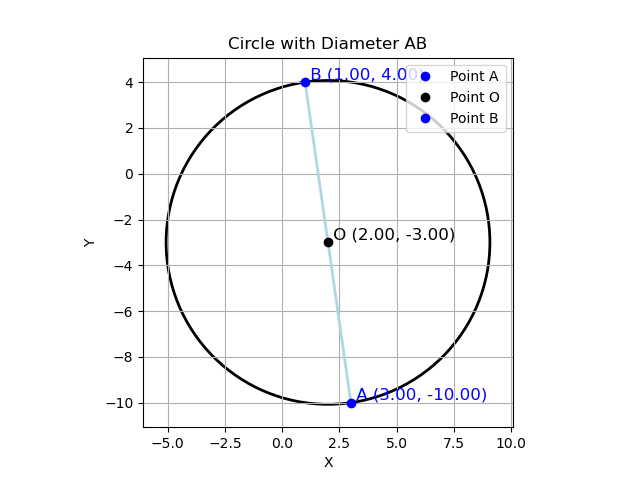
\includegraphics[width=0.7\columnwidth]{figs/Figure_1.png}
   \caption{Plot of the points and circle involved}
   \label{Fig}
\end{figure}

Code for plotting points and circle
\begin{lstlisting}
	codes/compute_b.c
	codes/plot_circle.py
\end{lstlisting}

\end{document}


